FPGA通常被归类为空间架构。它们受益于与使用指令集体系结构(ISA)的设备(包括大多数人更熟悉的CPU和GPU),从而形成非常不同的编码风格和并行形式。为了理解FPGA,我们将简要介绍基于ISA的加速器的一些思想,以便了解关键的区别。\par

就我们的目的而言,基于ISA的加速器设备可以执行许多不同的指令,一个或几个。这些指令通常比较简单,比如“从地址A的内存中加载数据”或“添加下组数字”。操作链串在一起形成一个程序,处理器就一条一条的执行指令。\par

基于ISA的加速器中,芯片的单个区域(或整个芯片)在每个时钟周期中执行来自程序的不同指令。这些指令在固定的硬件架构上执行,不同的硬件架构可以在不同的时间运行不同的指令,如图17-1所示。例如,输入加法的内存负载单元可能与输入减法的内存负载单元相同,同样的算术单元可能用于执行加法和减法指令。随着时间的推移,随着程序的执行,芯片上的硬件可以重用不同的指令。\par

\hspace*{\fill} \par %插入空行
图17-1 简单的基于ISA的(临时)处理:随着时间的推移重用硬件(区域)
\begin{center}
	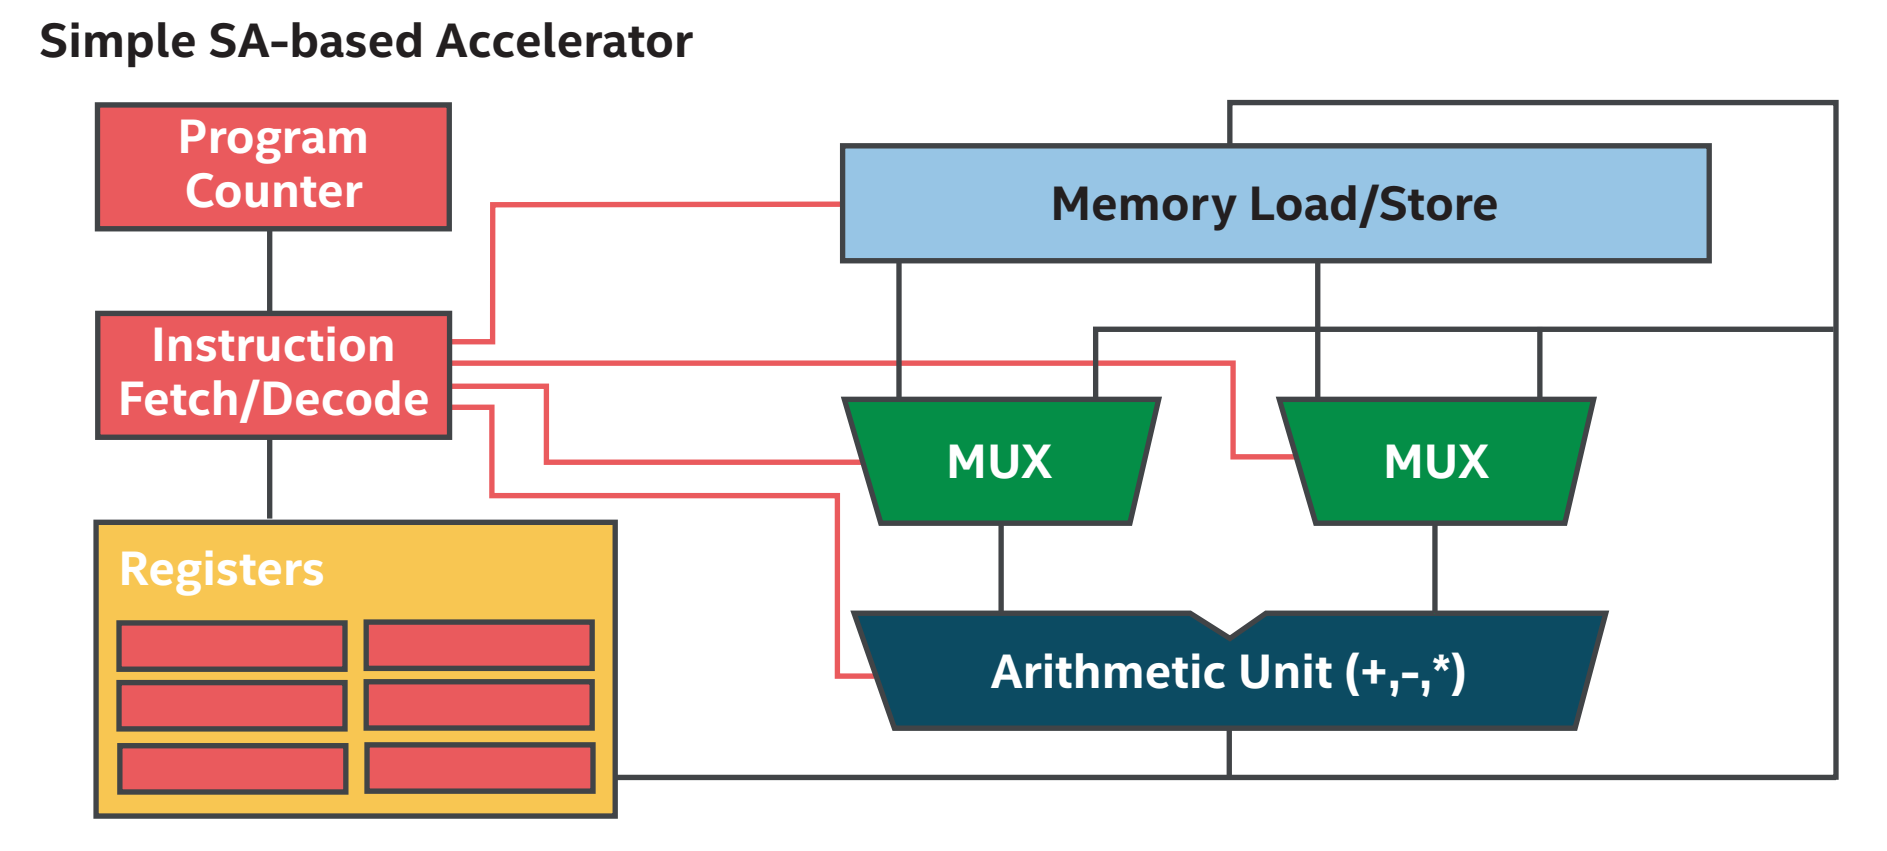
\includegraphics[width=1.0\textwidth]{content/chapter-17/images/2}
\end{center}

空间架构不同,它们不是基于在共享硬件上执行各种指令的机器,而是从相反的角度出发。程序空间在概念上把整个程序作为一个整体,并立即放在设备上执行,设备的不同区域在程序中执行不同的指令。在间架构中,专用硬件会接受到相应的指令,这些硬件可以与其他硬件同时执行(相同的时钟周期)。图17-2展示了这种思想,其为整个程序(本例中是一个非常简单的程序)的空间实现。\par

\hspace*{\fill} \par %插入空行
图17-2 空间处理:每个操作使用设备的不同区域
\begin{center}
	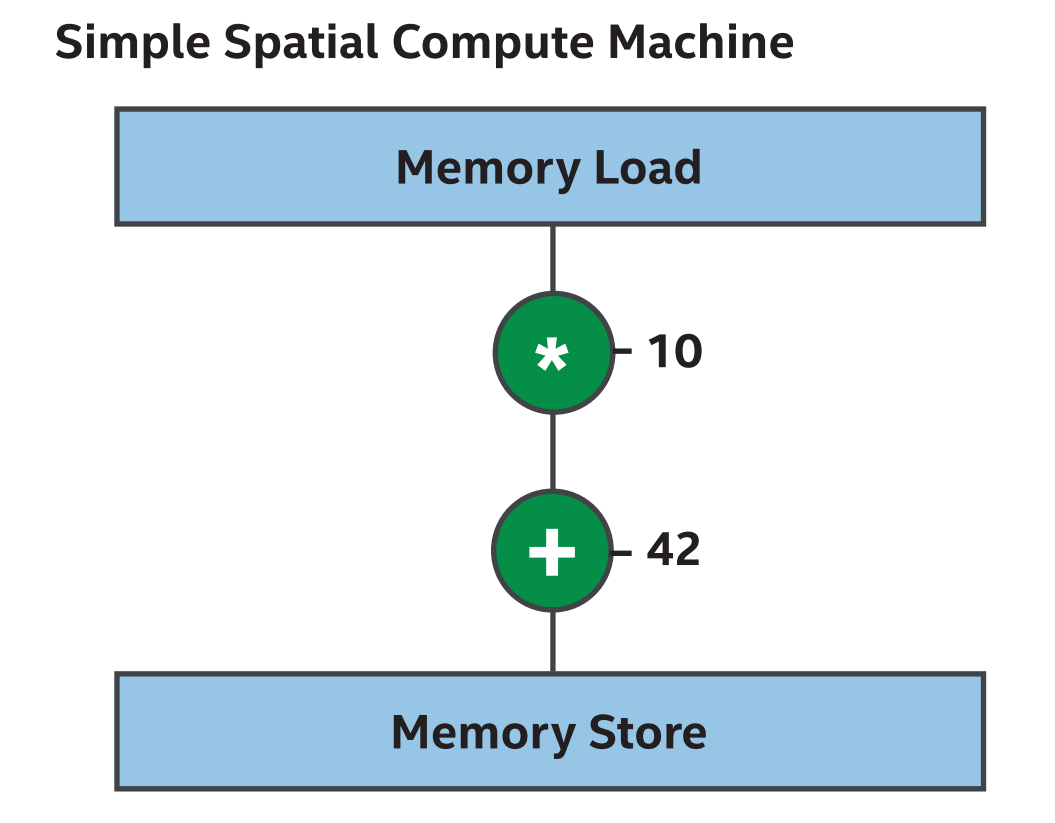
\includegraphics[width=1.0\textwidth]{content/chapter-17/images/3}
\end{center}

这个描程序过于简单,但它捕获在空间架构、程序的不同部分的不同部分设备上执行,而不是随着时间的推移发布到一组共享的通用硬件上。\par

由于FPGA的不同区域可以编程来执行不同的操作,一些与基于ISA的加速器相关联的硬件没必要的。例如,图17-2显示不再需要指令获取或解码单元、程序计数器或寄存器文件。空间体系结构将一条指令的输出与另一条指令的输入相连接,而不是将数据存储在寄存器文件中,这就是为什么空间体系结构通常称为数据流体系结构。\par

从介绍的FPGA映射中出现了几个明显的问题。首先,由于程序中的每条指令都占用设备空间面积一定的百分比,如果程序需要超过100\%的面积会发生什么?一些解决方案提供资源共享机制,使更大的程序能够以性能成本来适应,但FPGA确实有程序适应的概念。这既是优点也是缺点:\par

\begin{itemize}
	\item 好处:如果程序使用了FPGA上的大部分区域,并且在每个时钟周期中有足够的工作来保持所有硬件繁忙,由于极端的并行性,在设备上执行程序非常高效。更通用的体系结构可能在时钟周期中有大量未使用的硬件,而使用FPGA时,可以为特定应用程序完美地定制面积,不会浪费。这种定制可以让应用程序通过大规模并行运行得更快,通常可以提高能源利用的效率。
	\item 缺点:大型程序可能需要调整和重组才能适应设备。编译器的资源共享特性可以帮助解决这个问题,但通常会使性能下降,从而降低使用FPGA的好处。基于ISA的加速器是非常有效的资源共享实现——FPGA对计算有价值,主要是当应用程序可以利用大多数可用区域时。
\end{itemize}

极端的情况下,FPGA上的资源共享解决方案会看起来像基于ISA的加速器,但在可重构逻辑中构建。可重构逻辑导致相对于固定设计的开销大——因此,FPGA通常不作为实现ISA的方法。当应用程序能够利用资源来实现高效的数据流算法时,FPGA是最有利的,我们将在下一节中讨论这些算法。\par

\hspace*{\fill} \par %插入空行
\textbf{管道并行性}

图17-2中经常出现的另一个问题是,程序的空间实现如何与时钟频率相关,以及程序从开始到结束执行的速度。示例中,很容易相信数据可以很快地从内存中加载,执行乘法和加法运算,并将结果存储回内存中。随着程序变得越来越大,可能在FPGA设备上有成千上万的操作,所有的指令都要一个接一个地进行操作(操作通常取决于前一个操作产生的结果),考虑到每个操作带来的处理延迟,可能会花费大量的时间\par

如图17-3所示的空间体系结构中,操作之间的中间结果会随着时间的推移而更新(传播)。例如,load执行后将其结果传递给乘数器,乘数器的结果再传递给加法器,以此类推。一段时间后,中间数据一直传播到操作链的末端,最终结果可用或存储到内存中。\par

\hspace*{\fill} \par %插入空行
图17-3 空间计算实现的传播时间
\begin{center}
	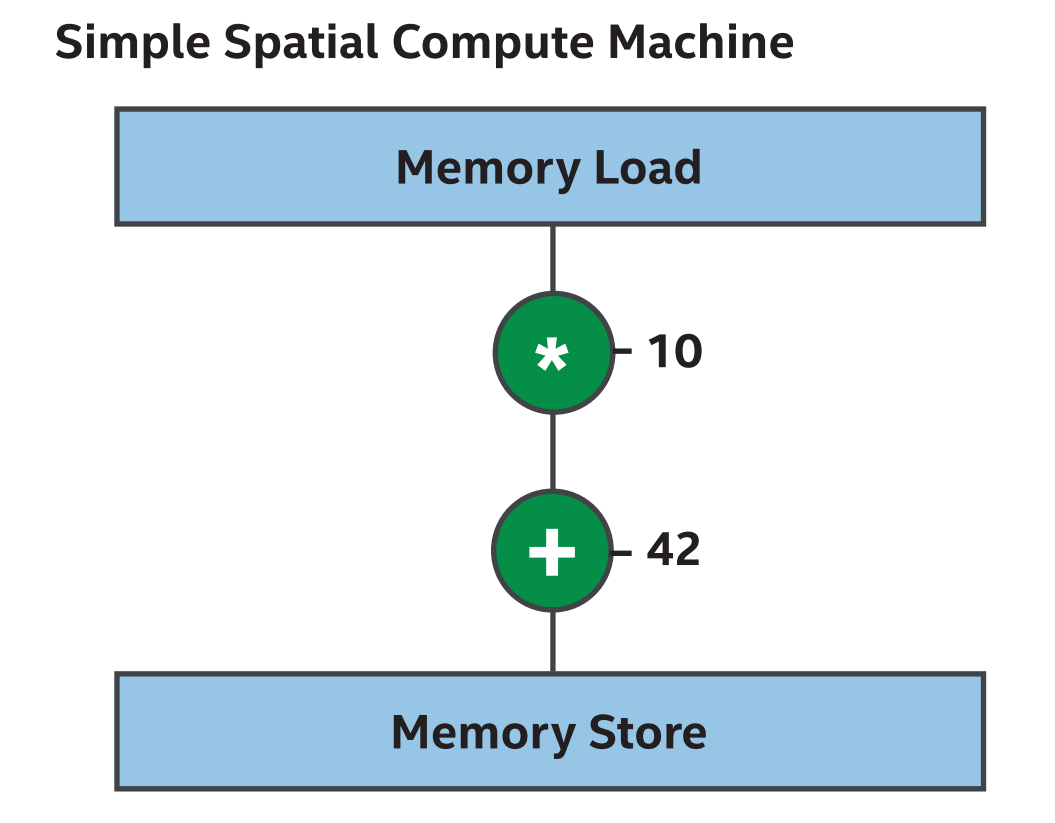
\includegraphics[width=1.0\textwidth]{content/chapter-17/images/3}
\end{center}

图17-3所示的空间实现是非常低效的,大多数硬件只在一小部分时间内执行有用的工作。大多数情况下,像乘法这样的操作要么等待加载中的新数据,要么保持其输出,以便让后续操作使用其结果。大多数空间编译器和实现通过流水线处理这种低效操作,这意味着单个程序的执行分散在多个时钟周期中。这是通过在一些操作之间插入寄存器(硬件中的数据存储原语)实现的,其中每个寄存器在一个时钟周期内保存一个二进制值。通过保存操作的输出结果,以便让下一个操作可以看到并对所保存的值进行操作,前一个操作可以自由地对不同的计算进行操作,而不会影响后续操作的输入。\par

算法流水线的目标是使每个操作(硬件单元)在每个时钟周期中处于繁忙状态。图17-4显示了前面简单示例的流水线实现。编译器会为我们完成所有的流水线和平衡工作!我们讨论这个主题是为了在接下来的章节中理解如何用工作填充流水线。\par

\hspace*{\fill} \par %插入空行
图17-4 计算流水线:各个阶段并行执行
\begin{center}
	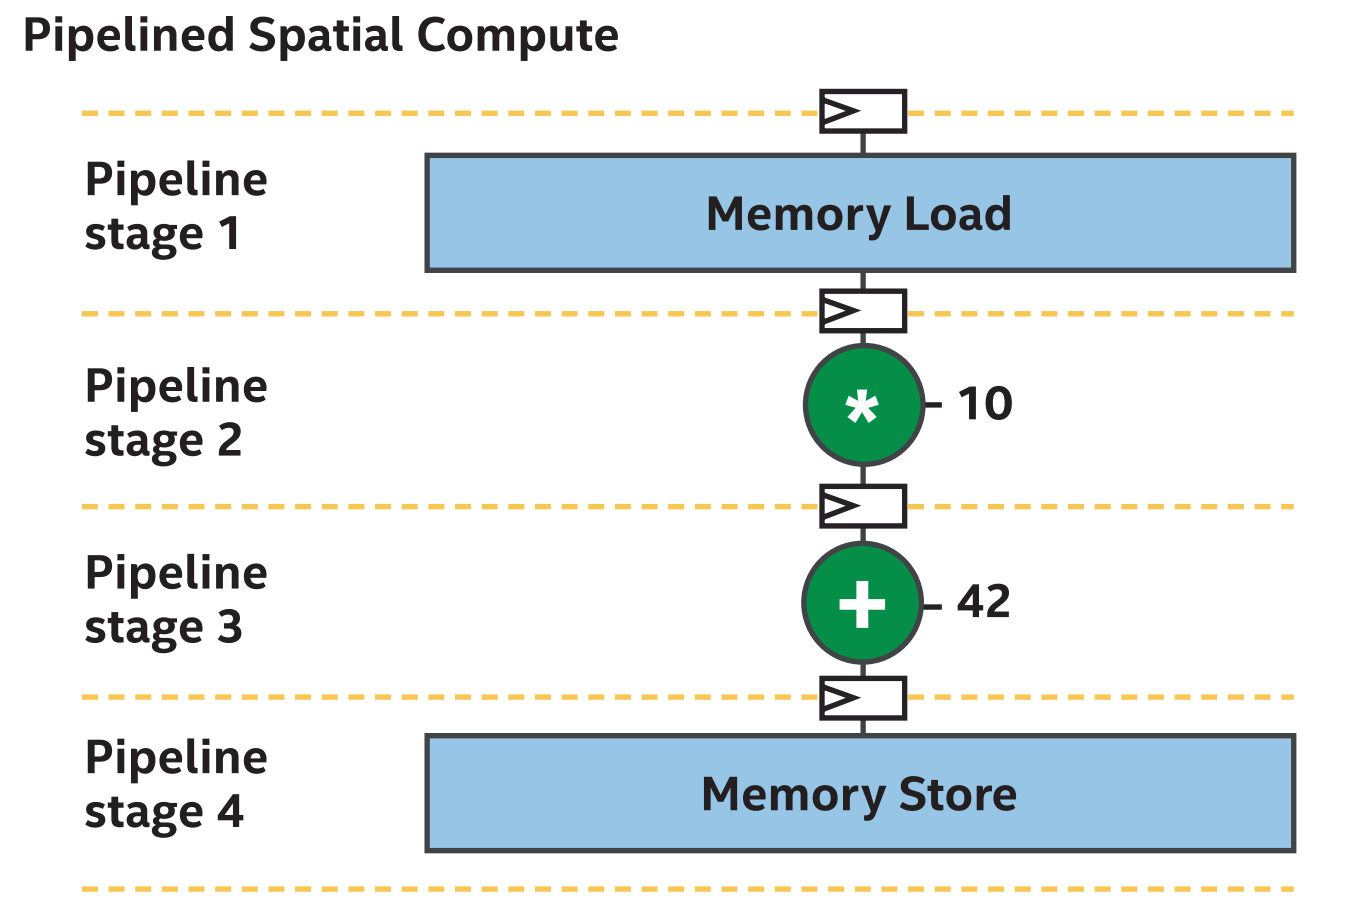
\includegraphics[width=1.0\textwidth]{content/chapter-17/images/5}
\end{center}

当空间实现流水线化,将以工厂装配线的方式变得非常高效。每个管道阶段只执行总体工作的一小部分,但它执行得很快,然后立即开始处理下一个工作单元。管道从开始到结束处理单个计算需要许多时钟周期,但是管道可以同时计算不同数据上的许多不同计算实例。\par

当足够多的工作在流水线中执行,超过足够多的连续时钟周期,那么每个流水线阶段和程序中的操作都可以在每个时钟周期中执行有用的工作,这意味着整个空间设备同时执行工作。这是空间架构的力量——整个设备可以在任何时候并行执行。我们称之为流水线并行性。\par

\begin{tcolorbox}[colback=red!5!white,colframe=red!75!black]
流水线并行是FPGA上用来实现性能的并行的主要形式。
\end{tcolorbox}

\begin{tcolorbox}[colback=blue!5!white,colframe=blue!75!black, title=自动型流水线]
在用于FPGA的DPC++的Intel实现中,以及用于FPGA的其他高级编程解决方案中,算法的流水线是由编译器自动执行。大致理解空间体系结构上的实现是很有用,因为这样就可以更容易地利用流水线并行性。流水线寄存器的使用平衡由编译器控制,而不是由开发控制。
\end{tcolorbox}

真正的程序和算法通常有控制流(例如,if/else结构),这会使程序的某些部分在一定百分比的时钟周期中处于非活动状态。FPGA编译器通常结合一个分支两边的硬件,尽可能减少浪费的空间面积,并在控制流发散期间最大化计算效率。这使得控制流分歧的成本大大降低,而且与其他方面(特别是向量化的体系结构)相比,开发上的关注点也更少。\par

\hspace*{\fill} \par %插入空行
\textbf{核心消费的芯片“区域”}

现有的实现中,DPC++应用程序中的每个内核都会生成一个空间管道,它消耗FPGA的一些资源(我们可以将其看作是设备上的空间或区域),如图17-5所示。\par

\hspace*{\fill} \par %插入空行
图17-5 同一个FPGA二进制文件中的多个内核:内核可以并发运行
\begin{center}
	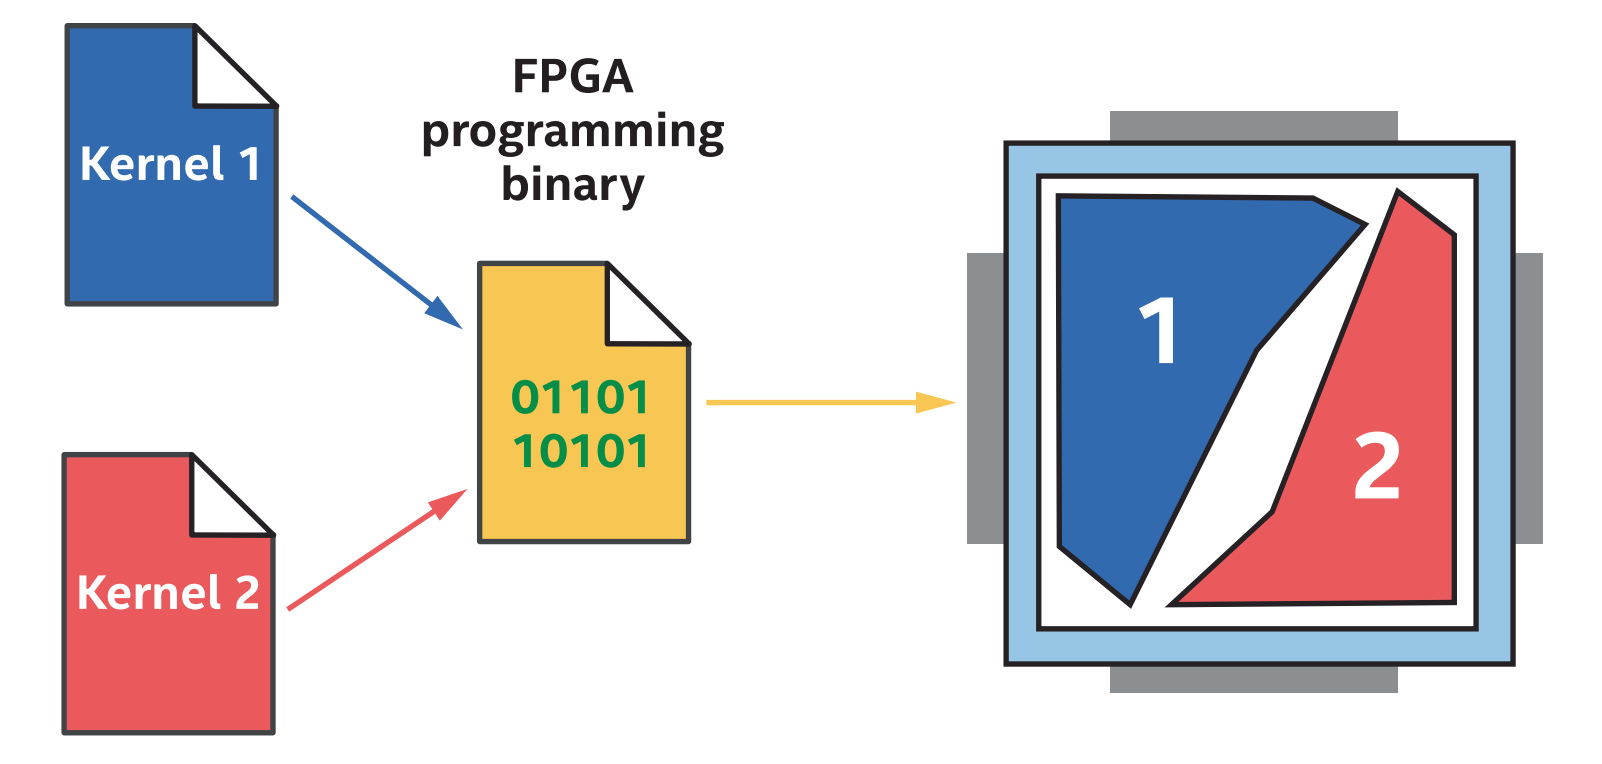
\includegraphics[width=1.0\textwidth]{content/chapter-17/images/6}
\end{center}

内核在设备上使用自己的区域,所以不同的内核可以并发执行。如果内核正在等待内存访问之类的操作,FPGA上的其他内核可以继续执行,因为芯片上的其他地方有独立的管道。这种思想形式上描述为内核之间的独立前向进程,是FPGA空间计算的关键属性。\par







